\documentclass[12pt]{article}
\usepackage[english]{babel}
\usepackage[utf8]{inputenc}
\usepackage[T1]{fontenc}
\usepackage{fancyhdr}
\usepackage{graphicx}
\usepackage{enumerate}
\usepackage{enumitem}
\usepackage{amsmath}
\usepackage{amssymb}
\usepackage{bm}
\usepackage{url}
\usepackage[dvipsnames]{xcolor}
\usepackage{booktabs}
\usepackage{longtable}
\usepackage{amsthm}
\usepackage[hidelinks]{hyperref}

% Formatting and Question/Answer structure match the Assignment 1 report.
\setlength{\parindent}{0cm}
\addtolength{\oddsidemargin}{-2cm}
\addtolength{\evensidemargin}{-2cm}
\setlength{\textwidth}{17.78cm}
\addtolength{\topmargin}{-2.25cm}
\setlength{\textheight}{23.24cm}
\setlength{\headheight}{30pt}
\addtolength{\parskip}{5mm}
\pagestyle{fancy}
%%%%% NEW MATH DEFINITIONS %%%%%

% Mark sections of captions for referring to divisions of figures
\newcommand{\figleft}{{\em (Left)}}
\newcommand{\figcenter}{{\em (Center)}}
\newcommand{\figright}{{\em (Right)}}
\newcommand{\figtop}{{\em (Top)}}
\newcommand{\figbottom}{{\em (Bottom)}}
\newcommand{\captiona}{{\em (a)}}
\newcommand{\captionb}{{\em (b)}}
\newcommand{\captionc}{{\em (c)}}
\newcommand{\captiond}{{\em (d)}}

% Highlight a newly defined term
\newcommand{\newterm}[1]{{\bf #1}}


% Figure reference, lower-case.
\def\figref#1{figure~\ref{#1}}
% Figure reference, capital. For start of sentence
\def\Figref#1{Figure~\ref{#1}}
\def\twofigref#1#2{figures \ref{#1} and \ref{#2}}
\def\quadfigref#1#2#3#4{figures \ref{#1}, \ref{#2}, \ref{#3} and \ref{#4}}
% Section reference, lower-case.
\def\secref#1{section~\ref{#1}}
% Section reference, capital.
\def\Secref#1{Section~\ref{#1}}
% Reference to two sections.
\def\twosecrefs#1#2{sections \ref{#1} and \ref{#2}}
% Reference to three sections.
\def\secrefs#1#2#3{sections \ref{#1}, \ref{#2} and \ref{#3}}
% Reference to an equation, lower-case.
\def\eqref#1{equation~\ref{#1}}
% Reference to an equation, upper case
\def\Eqref#1{Equation~\ref{#1}}
% A raw reference to an equation---avoid using if possible
\def\plaineqref#1{\ref{#1}}
% Reference to a chapter, lower-case.
\def\chapref#1{chapter~\ref{#1}}
% Reference to an equation, upper case.
\def\Chapref#1{Chapter~\ref{#1}}
% Reference to a range of chapters
\def\rangechapref#1#2{chapters\ref{#1}--\ref{#2}}
% Reference to an algorithm, lower-case.
\def\algref#1{algorithm~\ref{#1}}
% Reference to an algorithm, upper case.
\def\Algref#1{Algorithm~\ref{#1}}
\def\twoalgref#1#2{algorithms \ref{#1} and \ref{#2}}
\def\Twoalgref#1#2{Algorithms \ref{#1} and \ref{#2}}
% Reference to a part, lower case
\def\partref#1{part~\ref{#1}}
% Reference to a part, upper case
\def\Partref#1{Part~\ref{#1}}
\def\twopartref#1#2{parts \ref{#1} and \ref{#2}}

\def\ceil#1{\lceil #1 \rceil}
\def\floor#1{\lfloor #1 \rfloor}
\def\1{\bm{1}}
\newcommand{\train}{\mathcal{D}}
\newcommand{\valid}{\mathcal{D_{\mathrm{valid}}}}
\newcommand{\test}{\mathcal{D_{\mathrm{test}}}}

\def\eps{{\epsilon}}


% Random variables
\def\reta{{\textnormal{$\eta$}}}
\def\ra{{\textnormal{a}}}
\def\rb{{\textnormal{b}}}
\def\rc{{\textnormal{c}}}
\def\rd{{\textnormal{d}}}
\def\re{{\textnormal{e}}}
\def\rf{{\textnormal{f}}}
\def\rg{{\textnormal{g}}}
\def\rh{{\textnormal{h}}}
\def\ri{{\textnormal{i}}}
\def\rj{{\textnormal{j}}}
\def\rk{{\textnormal{k}}}
\def\rl{{\textnormal{l}}}
% rm is already a command, just don't name any random variables m
\def\rn{{\textnormal{n}}}
\def\ro{{\textnormal{o}}}
\def\rp{{\textnormal{p}}}
\def\rq{{\textnormal{q}}}
\def\rr{{\textnormal{r}}}
\def\rs{{\textnormal{s}}}
\def\rt{{\textnormal{t}}}
\def\ru{{\textnormal{u}}}
\def\rv{{\textnormal{v}}}
\def\rw{{\textnormal{w}}}
\def\rx{{\textnormal{x}}}
\def\ry{{\textnormal{y}}}
\def\rz{{\textnormal{z}}}

% Random vectors
\def\rvepsilon{{\mathbf{\epsilon}}}
\def\rvtheta{{\mathbf{\theta}}}
\def\rva{{\mathbf{a}}}
\def\rvb{{\mathbf{b}}}
\def\rvc{{\mathbf{c}}}
\def\rvd{{\mathbf{d}}}
\def\rve{{\mathbf{e}}}
\def\rvf{{\mathbf{f}}}
\def\rvg{{\mathbf{g}}}
\def\rvh{{\mathbf{h}}}
\def\rvu{{\mathbf{i}}}
\def\rvj{{\mathbf{j}}}
\def\rvk{{\mathbf{k}}}
\def\rvl{{\mathbf{l}}}
\def\rvm{{\mathbf{m}}}
\def\rvn{{\mathbf{n}}}
\def\rvo{{\mathbf{o}}}
\def\rvp{{\mathbf{p}}}
\def\rvq{{\mathbf{q}}}
\def\rvr{{\mathbf{r}}}
\def\rvs{{\mathbf{s}}}
\def\rvt{{\mathbf{t}}}
\def\rvu{{\mathbf{u}}}
\def\rvv{{\mathbf{v}}}
\def\rvw{{\mathbf{w}}}
\def\rvx{{\mathbf{x}}}
\def\rvy{{\mathbf{y}}}
\def\rvz{{\mathbf{z}}}

% Elements of random vectors
\def\erva{{\textnormal{a}}}
\def\ervb{{\textnormal{b}}}
\def\ervc{{\textnormal{c}}}
\def\ervd{{\textnormal{d}}}
\def\erve{{\textnormal{e}}}
\def\ervf{{\textnormal{f}}}
\def\ervg{{\textnormal{g}}}
\def\ervh{{\textnormal{h}}}
\def\ervi{{\textnormal{i}}}
\def\ervj{{\textnormal{j}}}
\def\ervk{{\textnormal{k}}}
\def\ervl{{\textnormal{l}}}
\def\ervm{{\textnormal{m}}}
\def\ervn{{\textnormal{n}}}
\def\ervo{{\textnormal{o}}}
\def\ervp{{\textnormal{p}}}
\def\ervq{{\textnormal{q}}}
\def\ervr{{\textnormal{r}}}
\def\ervs{{\textnormal{s}}}
\def\ervt{{\textnormal{t}}}
\def\ervu{{\textnormal{u}}}
\def\ervv{{\textnormal{v}}}
\def\ervw{{\textnormal{w}}}
\def\ervx{{\textnormal{x}}}
\def\ervy{{\textnormal{y}}}
\def\ervz{{\textnormal{z}}}

% Random matrices
\def\rmA{{\mathbf{A}}}
\def\rmB{{\mathbf{B}}}
\def\rmC{{\mathbf{C}}}
\def\rmD{{\mathbf{D}}}
\def\rmE{{\mathbf{E}}}
\def\rmF{{\mathbf{F}}}
\def\rmG{{\mathbf{G}}}
\def\rmH{{\mathbf{H}}}
\def\rmI{{\mathbf{I}}}
\def\rmJ{{\mathbf{J}}}
\def\rmK{{\mathbf{K}}}
\def\rmL{{\mathbf{L}}}
\def\rmM{{\mathbf{M}}}
\def\rmN{{\mathbf{N}}}
\def\rmO{{\mathbf{O}}}
\def\rmP{{\mathbf{P}}}
\def\rmQ{{\mathbf{Q}}}
\def\rmR{{\mathbf{R}}}
\def\rmS{{\mathbf{S}}}
\def\rmT{{\mathbf{T}}}
\def\rmU{{\mathbf{U}}}
\def\rmV{{\mathbf{V}}}
\def\rmW{{\mathbf{W}}}
\def\rmX{{\mathbf{X}}}
\def\rmY{{\mathbf{Y}}}
\def\rmZ{{\mathbf{Z}}}

% Elements of random matrices
\def\ermA{{\textnormal{A}}}
\def\ermB{{\textnormal{B}}}
\def\ermC{{\textnormal{C}}}
\def\ermD{{\textnormal{D}}}
\def\ermE{{\textnormal{E}}}
\def\ermF{{\textnormal{F}}}
\def\ermG{{\textnormal{G}}}
\def\ermH{{\textnormal{H}}}
\def\ermI{{\textnormal{I}}}
\def\ermJ{{\textnormal{J}}}
\def\ermK{{\textnormal{K}}}
\def\ermL{{\textnormal{L}}}
\def\ermM{{\textnormal{M}}}
\def\ermN{{\textnormal{N}}}
\def\ermO{{\textnormal{O}}}
\def\ermP{{\textnormal{P}}}
\def\ermQ{{\textnormal{Q}}}
\def\ermR{{\textnormal{R}}}
\def\ermS{{\textnormal{S}}}
\def\ermT{{\textnormal{T}}}
\def\ermU{{\textnormal{U}}}
\def\ermV{{\textnormal{V}}}
\def\ermW{{\textnormal{W}}}
\def\ermX{{\textnormal{X}}}
\def\ermY{{\textnormal{Y}}}
\def\ermZ{{\textnormal{Z}}}

% Vectors
\def\vzero{{\bm{0}}}
\def\vone{{\bm{1}}}
\def\vmu{{\bm{\mu}}}
\def\vtheta{{\bm{\theta}}}
\def\va{{\bm{a}}}
\def\vb{{\bm{b}}}
\def\vc{{\bm{c}}}
\def\vd{{\bm{d}}}
\def\ve{{\bm{e}}}
\def\vf{{\bm{f}}}
\def\vg{{\bm{g}}}
\def\vh{{\bm{h}}}
\def\vi{{\bm{i}}}
\def\vj{{\bm{j}}}
\def\vk{{\bm{k}}}
\def\vl{{\bm{l}}}
\def\vm{{\bm{m}}}
\def\vn{{\bm{n}}}
\def\vo{{\bm{o}}}
\def\vp{{\bm{p}}}
\def\vq{{\bm{q}}}
\def\vr{{\bm{r}}}
\def\vs{{\bm{s}}}
\def\vt{{\bm{t}}}
\def\vu{{\bm{u}}}
\def\vv{{\bm{v}}}
\def\vw{{\bm{w}}}
\def\vx{{\bm{x}}}
\def\vy{{\bm{y}}}
\def\vz{{\bm{z}}}

% Elements of vectors
\def\evalpha{{\alpha}}
\def\evbeta{{\beta}}
\def\evepsilon{{\epsilon}}
\def\evlambda{{\lambda}}
\def\evomega{{\omega}}
\def\evmu{{\mu}}
\def\evpsi{{\psi}}
\def\evsigma{{\sigma}}
\def\evtheta{{\theta}}
\def\eva{{a}}
\def\evb{{b}}
\def\evc{{c}}
\def\evd{{d}}
\def\eve{{e}}
\def\evf{{f}}
\def\evg{{g}}
\def\evh{{h}}
\def\evi{{i}}
\def\evj{{j}}
\def\evk{{k}}
\def\evl{{l}}
\def\evm{{m}}
\def\evn{{n}}
\def\evo{{o}}
\def\evp{{p}}
\def\evq{{q}}
\def\evr{{r}}
\def\evs{{s}}
\def\evt{{t}}
\def\evu{{u}}
\def\evv{{v}}
\def\evw{{w}}
\def\evx{{x}}
\def\evy{{y}}
\def\evz{{z}}

% Matrix
\def\mA{{\bm{A}}}
\def\mB{{\bm{B}}}
\def\mC{{\bm{C}}}
\def\mD{{\bm{D}}}
\def\mE{{\bm{E}}}
\def\mF{{\bm{F}}}
\def\mG{{\bm{G}}}
\def\mH{{\bm{\text{\textbf{H}}}}}
\def\mI{{\bm{I}}}
\def\mJ{{\bm{J}}}
\def\mK{{\bm{K}}}
\def\mL{{\bm{L}}}
\def\mM{{\bm{M}}}
\def\mN{{\bm{N}}}
\def\mO{{\bm{O}}}
\def\mP{{\bm{P}}}
\def\mQ{{\bm{Q}}}
\def\mR{{\bm{R}}}
\def\mS{{\bm{S}}}
\def\mT{{\bm{T}}}
\def\mU{{\bm{U}}}
\def\mV{{\bm{V}}}
\def\mW{{\bm{W}}}
\def\mX{{\bm{X}}}
\def\mY{{\bm{Y}}}
\def\mZ{{\bm{Z}}}
\def\mBeta{{\bm{\beta}}}
\def\mPhi{{\bm{\Phi}}}
\def\mLambda{{\bm{\Lambda}}}
\def\mSigma{{\bm{\Sigma}}}

% Tensor
\DeclareMathAlphabet{\mathsfit}{\encodingdefault}{\sfdefault}{m}{sl}
\SetMathAlphabet{\mathsfit}{bold}{\encodingdefault}{\sfdefault}{bx}{n}
\newcommand{\tens}[1]{\bm{\mathsfit{#1}}}
\def\tA{{\tens{A}}}
\def\tB{{\tens{B}}}
\def\tC{{\tens{C}}}
\def\tD{{\tens{D}}}
\def\tE{{\tens{E}}}
\def\tF{{\tens{F}}}
\def\tG{{\tens{G}}}
\def\tH{{\tens{H}}}
\def\tI{{\tens{I}}}
\def\tJ{{\tens{J}}}
\def\tK{{\tens{K}}}
\def\tL{{\tens{L}}}
\def\tM{{\tens{M}}}
\def\tN{{\tens{N}}}
\def\tO{{\tens{O}}}
\def\tP{{\tens{P}}}
\def\tQ{{\tens{Q}}}
\def\tR{{\tens{R}}}
\def\tS{{\tens{S}}}
\def\tT{{\tens{T}}}
\def\tU{{\tens{U}}}
\def\tV{{\tens{V}}}
\def\tW{{\tens{W}}}
\def\tX{{\tens{X}}}
\def\tY{{\tens{Y}}}
\def\tZ{{\tens{Z}}}


% Graph
\def\gA{{\mathcal{A}}}
\def\gB{{\mathcal{B}}}
\def\gC{{\mathcal{C}}}
\def\gD{{\mathcal{D}}}
\def\gE{{\mathcal{E}}}
\def\gF{{\mathcal{F}}}
\def\gG{{\mathcal{G}}}
\def\gH{{\mathcal{H}}}
\def\gI{{\mathcal{I}}}
\def\gJ{{\mathcal{J}}}
\def\gK{{\mathcal{K}}}
\def\gL{{\mathcal{L}}}
\def\gM{{\mathcal{M}}}
\def\gN{{\mathcal{N}}}
\def\gO{{\mathcal{O}}}
\def\gP{{\mathcal{P}}}
\def\gQ{{\mathcal{Q}}}
\def\gR{{\mathcal{R}}}
\def\gS{{\mathcal{S}}}
\def\gT{{\mathcal{T}}}
\def\gU{{\mathcal{U}}}
\def\gV{{\mathcal{V}}}
\def\gW{{\mathcal{W}}}
\def\gX{{\mathcal{X}}}
\def\gY{{\mathcal{Y}}}
\def\gZ{{\mathcal{Z}}}

% Sets
\def\sA{{\mathbb{A}}}
\def\sB{{\mathbb{B}}}
\def\sC{{\mathbb{C}}}
\def\sD{{\mathbb{D}}}
% Don't use a set called E, because this would be the same as our symbol
% for expectation.
\def\sF{{\mathbb{F}}}
\def\sG{{\mathbb{G}}}
\def\sH{{\mathbb{H}}}
\def\sI{{\mathbb{I}}}
\def\sJ{{\mathbb{J}}}
\def\sK{{\mathbb{K}}}
\def\sL{{\mathbb{L}}}
\def\sM{{\mathbb{M}}}
\def\sN{{\mathbb{N}}}
\def\sO{{\mathbb{O}}}
\def\sP{{\mathbb{P}}}
\def\sQ{{\mathbb{Q}}}
\def\sR{{\mathbb{R}}}
\def\sS{{\mathbb{S}}}
\def\sT{{\mathbb{T}}}
\def\sU{{\mathbb{U}}}
\def\sV{{\mathbb{V}}}
\def\sW{{\mathbb{W}}}
\def\sX{{\mathbb{X}}}
\def\sY{{\mathbb{Y}}}
\def\sZ{{\mathbb{Z}}}

% Entries of a matrix
\def\emLambda{{\Lambda}}
\def\emA{{A}}
\def\emB{{B}}
\def\emC{{C}}
\def\emD{{D}}
\def\emE{{E}}
\def\emF{{F}}
\def\emG{{G}}
\def\emH{{H}}
\def\emI{{I}}
\def\emJ{{J}}
\def\emK{{K}}
\def\emL{{L}}
\def\emM{{M}}
\def\emN{{N}}
\def\emO{{O}}
\def\emP{{P}}
\def\emQ{{Q}}
\def\emR{{R}}
\def\emS{{S}}
\def\emT{{T}}
\def\emU{{U}}
\def\emV{{V}}
\def\emW{{W}}
\def\emX{{X}}
\def\emY{{Y}}
\def\emZ{{Z}}
\def\emSigma{{\Sigma}}

% entries of a tensor
% Same font as tensor, without \bm wrapper
\newcommand{\etens}[1]{\mathsfit{#1}}
\def\etLambda{{\etens{\Lambda}}}
\def\etA{{\etens{A}}}
\def\etB{{\etens{B}}}
\def\etC{{\etens{C}}}
\def\etD{{\etens{D}}}
\def\etE{{\etens{E}}}
\def\etF{{\etens{F}}}
\def\etG{{\etens{G}}}
\def\etH{{\etens{H}}}
\def\etI{{\etens{I}}}
\def\etJ{{\etens{J}}}
\def\etK{{\etens{K}}}
\def\etL{{\etens{L}}}
\def\etM{{\etens{M}}}
\def\etN{{\etens{N}}}
\def\etO{{\etens{O}}}
\def\etP{{\etens{P}}}
\def\etQ{{\etens{Q}}}
\def\etR{{\etens{R}}}
\def\etS{{\etens{S}}}
\def\etT{{\etens{T}}}
\def\etU{{\etens{U}}}
\def\etV{{\etens{V}}}
\def\etW{{\etens{W}}}
\def\etX{{\etens{X}}}
\def\etY{{\etens{Y}}}
\def\etZ{{\etens{Z}}}

% The true underlying data generating distribution
\newcommand{\pdata}{p_{\rm{data}}}
% The empirical distribution defined by the training set
\newcommand{\ptrain}{\hat{p}_{\rm{data}}}
\newcommand{\Ptrain}{\hat{P}_{\rm{data}}}
% The model distribution
\newcommand{\pmodel}{p_{\rm{model}}}
\newcommand{\Pmodel}{P_{\rm{model}}}
\newcommand{\ptildemodel}{\tilde{p}_{\rm{model}}}
% Stochastic autoencoder distributions
\newcommand{\pencode}{p_{\rm{encoder}}}
\newcommand{\pdecode}{p_{\rm{decoder}}}
\newcommand{\precons}{p_{\rm{reconstruct}}}

\newcommand{\laplace}{\mathrm{Laplace}} % Laplace distribution

\newcommand{\E}{\mathbb{E}}
\newcommand{\Ls}{\mathcal{L}}
\newcommand{\R}{\mathbb{R}}
\newcommand{\emp}{\tilde{p}}
\newcommand{\lr}{\alpha}
\newcommand{\reg}{\lambda}
\newcommand{\rect}{\mathrm{rectifier}}
\newcommand{\softmax}{\mathrm{softmax}}
\newcommand{\sigmoid}{\sigma}
\newcommand{\softplus}{\zeta}
\newcommand{\KL}{D_{\mathrm{KL}}}
\newcommand{\Var}{\mathrm{Var}}
\newcommand{\standarderror}{\mathrm{SE}}
\newcommand{\Cov}{\mathrm{Cov}}
% Wolfram Mathworld says $L^2$ is for function spaces and $\ell^2$ is for vectors
% But then they seem to use $L^2$ for vectors throughout the site, and so does
% wikipedia.
\newcommand{\normlzero}{L^0}
\newcommand{\normlone}{L^1}
\newcommand{\normltwo}{L^2}
\newcommand{\normlp}{L^p}
\newcommand{\normmax}{L^\infty}

\newcommand{\parents}{Pa} % See usage in notation.tex. Chosen to match Daphne's book.

\DeclareMathOperator*{\argmax}{arg\,max}
\DeclareMathOperator*{\argmin}{arg\,min}

\DeclareMathOperator{\sign}{sign}
\DeclareMathOperator{\Tr}{Tr}
\let\ab\allowbreak


%%% new
\newcommand{\diag}{\mathop{\mathrm{diag}}\nolimits}
\usepackage{cancel}
\newcommand{\ttt}[1]{\texttt{#1}}

\newif\ifexercise
\exercisetrue
\newif\ifsolution
\solutiontrue
\theoremstyle{definition}
\newtheorem{exercise}{Question}
\newtheorem{answer}{Answer}
\newcommand{\Exercise}[1]{\ifexercise#1\fi}
\definecolor{answer}{rgb}{0.00, 0.12, 0.60}
\newcommand{\Answer}[1]{%
  \ifsolution
    \begingroup
    \color{answer}
    \begin{answer}#1\end{answer}
    \endgroup
  \fi
}
\setlist[enumerate,1]{leftmargin=*, label=\arabic*.}
\newcommand{\ToComplete}{\textit{[To be completed from notebook outputs.]}}
\newcommand{\Blank}{\textemdash}
\newcommand{\FigurePlaceholder}[1]{%
  \par\smallskip\noindent
  \fbox{\parbox[c][2.2cm][c]{0.94\linewidth}{\centering\itshape #1}}
  \par\smallskip
}
\graphicspath{{report-assets/}}

\begin{document}
\fancyhead{}
\fancyfoot{}
\fancyhead[L]{\begin{tabular}[b]{l}
  IFT6135-A2026 \\
  Prof: Aishwarya Agrawal
\end{tabular}}
\fancyhead[R]{\begin{tabular}[b]{r}
  Assignment 2 -- Programming Report \\
  Recurrent Neural Networks and Transformers
\end{tabular}}
\fancyfoot[C]{\thepage\quad -- Do not distribute --}

\textbf{Due Date: November 15th, 2026 at 11:00 pm}

\textbf{Student name:} Marsel Bakashov\par
\textbf{Student number:} 20216284\par
\textbf{Google Colab notebook (executed, publicly accessible):} \url{https://colab.research.google.com/drive/1mkrZt_VTwP_8uRPqOL60d1Pw37U7fWXo?usp=sharing}\par

% Report-only skeleton. Code is submitted in the single assignment notebook.
% Insert actual notebook outputs and interpretations; do not invent results.

\begin{exercise}[50] \textbf{Learning to Update Memory with LSTMs}
\Exercise{
\subsection*{Part 2: Training and memory analysis (20 points)}
Use the provided training script and seed 6135. The configuration is
20 epochs, batch size 128, Adam with learning rate 0.003, and gradient-norm
clipping at 1.0. Do not add layers or perform a hyperparameter search.
Select the checkpoint with the lowest validation cross-entropy, keeping
the earlier epoch in a tie. Do not use a test set to select a checkpoint.
CPU execution is supported. The provided evaluation script uses \texttt{model.eval()} and \texttt{torch.no\_grad()} without updating model parameters.

\begin{enumerate}[label=\textbf{1.2.\arabic*}, leftmargin=*]
\item \textbf{Training and evaluation (6 points).} Report training and
validation loss and accuracy curves (2), the selected epoch and selection
rule (2), and the hardware, software versions, total training/validation
time, and model parameter count (2). Use the supplied notebook outputs directly; no additional experiments are required. Save the supplied run outputs.

\item \textbf{Memory analysis (8 points).} Evaluate the same selected
checkpoint, without retraining, on the 15 supplied conditions
$D\in\{0,4,8,16,32\}$ and $R\in\{1,2,3\}$, with 360 examples per
condition. Here the queried key's final update is balanced across positions
2, 3, and 4 in every condition. Thus its position distribution is the same
when comparing different $R$, without exposing one fixed answer position.
Report an accuracy table and plot accuracy
against $D$, with one curve per $R$ (3). For $R\geq2$, also report the
\emph{stale-value rate}: the fraction of all examples in that condition
whose prediction equals the immediately previous value of the queried key
(2). Report this rate as not applicable for $R=1$.
In one short paragraph (about 3--5 sentences), explain the patterns and distinguish observed performance from a guaranteed
memory capability (3). Identify which distractor lengths were absent from
training. Do not assume that every increase in $D$ or $R$ must reduce accuracy. Differences across $R$ should be interpreted descriptively, since earlier update patterns and spacing also vary. These results concern distractors after all updates, not distractors interleaved with updates.

\item \textbf{Failure analysis (6 points).} Show two actual errors when at least two exist
across the test conditions, using the exported example IDs, decoded
sequences, true labels, predictions, and previous values (3). Prefer different error types when available; both types are not required.
Distinguish stale-value errors from other errors and give a plausible
explanation connected to retaining and updating memory in 2--3 sentences per example (3). You do not need to prove the internal cause.
If fewer than two errors exist, show all available errors and state their
number; if none exist, show two correct examples and discuss the limits of
this evidence. Failure to make errors does not lose marks.
\end{enumerate}
}
\end{exercise}

\clearpage
\Answer{
\leavevmode\par
\begin{enumerate}[label=\textbf{1.2.\arabic*}, leftmargin=*]
    \item \textbf{Training and evaluation.}\par
    \begin{center}
    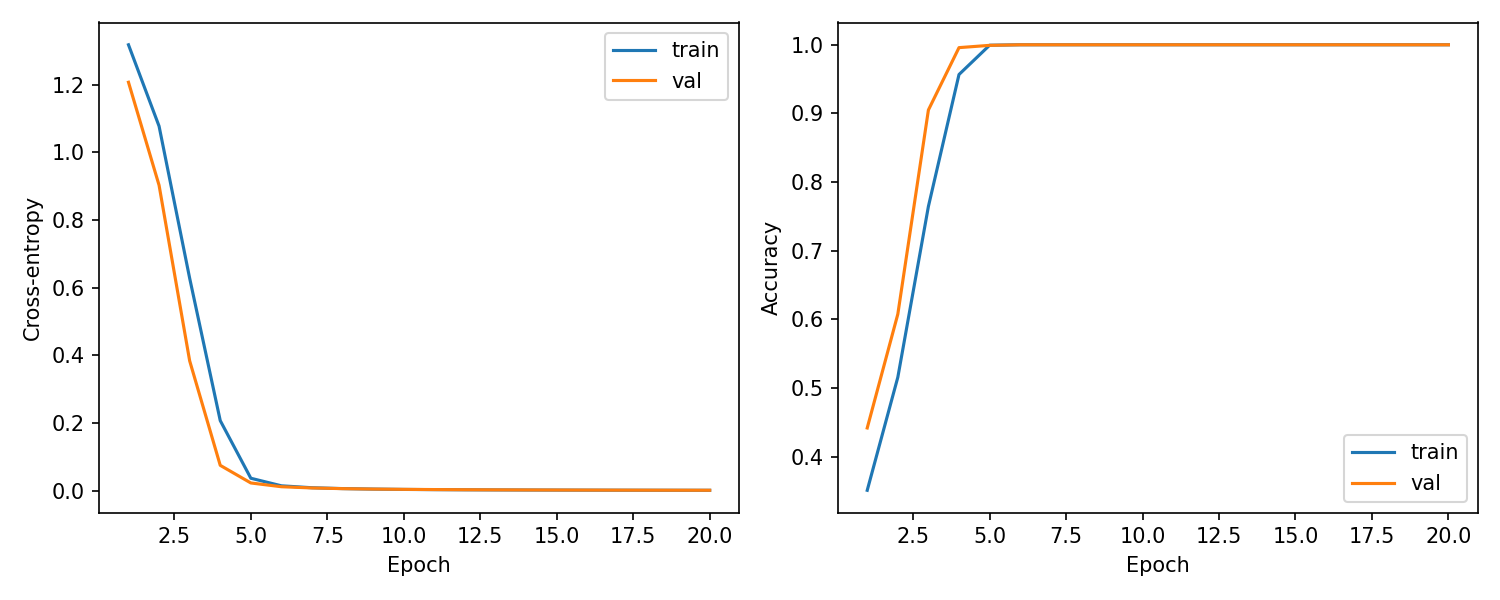
\includegraphics[width=\linewidth]{q1_learning_curves.png}\\
    {\small Training and validation cross-entropy and accuracy by epoch.}
    \end{center}
    The selected checkpoint is from \textbf{epoch 20}, chosen by lowest
    validation cross-entropy; an earlier epoch is retained in case of a tie.
    Validation accuracy reaches 100\% around epoch 5, but the validation
    cross-entropy keeps decreasing slowly until the end, so the lowest value
    is at the last epoch.

    \textbf{Hardware:} NVIDIA Tesla T4 GPU.\par
    \textbf{Software:} Python 3.13.16; PyTorch 2.14.1+cu130;
    Linux 6.6.159+ (x86\_64, glibc 2.39).\par
    \textbf{Total training and validation time:} 18.74 seconds.\par
    \textbf{Model parameter count:} 25,732.

    \item \textbf{Memory analysis.}\par
    Accuracy and stale-value rate for the selected checkpoint. Each
    condition contains 360 examples; stale-value rate is not applicable
    when $R=1$.
    \begin{center}
    \begin{tabular}{cccccc}
    \toprule
    $D$ & \multicolumn{3}{c}{Accuracy} & \multicolumn{2}{c}{Stale-value rate} \\
    \cmidrule(lr){2-4}\cmidrule(lr){5-6}
    & $R=1$ & $R=2$ & $R=3$ & $R=2$ & $R=3$ \\
    \midrule
    0  & 1.0000 & 1.0000 & 1.0000 & 0.0000 & 0.0000 \\
    4  & 1.0000 & 1.0000 & 1.0000 & 0.0000 & 0.0000 \\
    8  & 1.0000 & 0.9972 & 1.0000 & 0.0028 & 0.0000 \\
    16 & 1.0000 & 0.9972 & 1.0000 & 0.0028 & 0.0000 \\
    32 & 0.9722 & 0.9639 & 0.9611 & 0.0111 & 0.0250 \\
    \bottomrule
    \end{tabular}
    \end{center}
    \begin{center}
    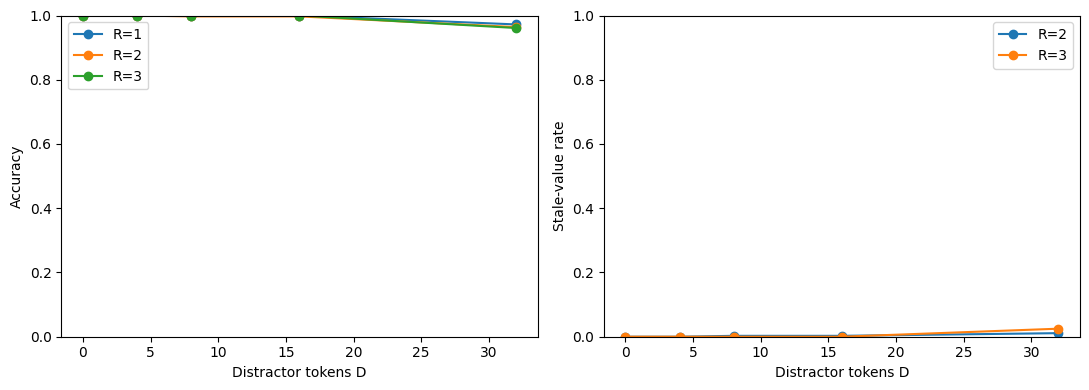
\includegraphics[width=\linewidth]{q1_memory_analysis.png}\\
    {\small Accuracy and stale-value rate versus distractor length.}
    \end{center}
    Accuracy stays at or above 99.72\% up to $D=16$, then drops to
    96.11--97.22\% at $D=32$. The lengths $D=16$ and $D=32$ were never seen in
    training ($D\in\{0,2,4,8\}$), so the model extrapolates well to twice the
    longest training length but starts to fail at four times. The trend is not
    monotone in $R$: $R=3$ is perfect at $D=8$ and $16$ while $R=2$ makes one
    error, but at $D=32$ stale values explain about 64\% of the $R=3$ errors
    ($0.0250/0.0389$) against about 31\% for $R=2$ ($0.0111/0.0361$). This is
    observed performance on these 360 examples per condition, not a
    guaranteed memory: nothing shows that it holds for longer sequences or
    when distractors are placed between the updates.

    \item \textbf{Failure analysis.}\par
    \textbf{Example 1 -- stale-value error} (\texttt{test-d8-r2-00151}):
    \begin{quote}\ttfamily\small
    A=2 $\to$ A=2 $\to$ B=1 $\to$ C=3 $\to$ B=3 $\to$ C=3
    $\to$ D0 $\to$ D0 $\to$ D1 $\to$ D2 $\to$ D3 $\to$ D3
    $\to$ D1 $\to$ D3 $\to$ QUERY B
    \end{quote}
    Target: 3; prediction: 1; previous value: 1. This is a stale-value
    error: the model answers with B's earlier value instead of its latest
    update. A plausible explanation is that when B=3 arrived, the input and
    forget gates only partly overwrote the old value in the cell state, and
    the remaining trace of B=1 won after the eight distractors.

    \textbf{Example 2 -- other error} (\texttt{test-d32-r1-00026}):
    \begin{quote}\ttfamily\small
    A=1 $\to$ C=2 $\to$ A=0 $\to$ C=2 $\to$ B=0 $\to$ C=0
    $\to$ D3 $\to$ D3 $\to$ D0 $\to$ D2 $\to$ D1 $\to$ D0
    $\to$ D2 $\to$ D2 $\to$ D2 $\to$ D3 $\to$ D1 $\to$ D2
    $\to$ D1 $\to$ D2 $\to$ D2 $\to$ D0 $\to$ D3 $\to$ D0
    $\to$ D0 $\to$ D1 $\to$ D2 $\to$ D2 $\to$ D1 $\to$ D0
    $\to$ D3 $\to$ D0 $\to$ D0 $\to$ D0 $\to$ D0 $\to$ D1
    $\to$ D1 $\to$ D1 $\to$ QUERY B
    \end{quote}
    Target: 0; prediction: 1; previous value: not applicable ($R=1$).
    This is not a stale-value error, since B has only one update. The
    sequence has 32 distractors, four times more than any training sequence,
    and since the forget gate is never exactly 1, the stored value of B can
    slowly drift until a wrong value wins.
\end{enumerate}
}

\clearpage
\begin{exercise}[50] \textbf{Word-Level vs.\ Sentence-Level Representation Learning with Transformers}
\Exercise{
\subsection*{Part 3: Evaluation (14 points)}
Answer in your PDF report. All metrics, tables and plots are computed by
provided functions in the notebook. Include the outputs each question asks for.

The notebook compares the four models with two metrics:
\begin{itemize}
  \item \textbf{Masked-word accuracy}: 15\% of the words of the 5,000 held-out sentences are
        masked as in Part 1, and the accuracy is the fraction of masked positions where the MLM head's top guess,
        $\arg\max_w \ell_{t,w}$, is the original word.
  \item \textbf{Cosine of similar vs.\ dissimilar pairs}: let $\mathcal{S}$ be the 338 STS-B
        pairs rated 4 or more (similar) and $\mathcal{D}$ the 308 pairs rated 1 or less (dissimilar). For a pair of
        sentences with embeddings $(z,z')$, the notebook reports the mean cosines and their gap,
        \[
          \overline{\cos}_{\mathcal{S}} = \frac{1}{|\mathcal{S}|} \sum_{(z,z')\in\mathcal{S}} \cos(z,z'), \quad
          \overline{\cos}_{\mathcal{D}} = \frac{1}{|\mathcal{D}|} \sum_{(z,z')\in\mathcal{D}} \cos(z,z'), \quad
          \text{gap}=\overline{\cos}_{\mathcal{S}}-\overline{\cos}_{\mathcal{D}}.
        \]
        A good sentence embedding gives similar pairs a much higher cosine than dissimilar ones: a large gap.
\end{itemize}

\begin{enumerate}[label=\textbf{2.3.\arabic*}, leftmargin=*]
  \item \textbf{Training (2 pts).} Include the loss curves (training and validation loss of each model against
  training steps).
  \begin{enumerate}[label=(\alph*)]
    \item Did any of the three models overfit? Justify your answer using the curves.
  \end{enumerate}

  \item \textbf{Word level vs.\ sentence level (7 pts).} Include the results table, the masked-word accuracy plot,
  the cosine plot, and the fill-in-the-blank output for the two given sentences and one sentence of your own.
  \begin{enumerate}[label=(\alph*)]
    \item Which model has the highest masked-word accuracy? Explain. [2 sentences max.]
    \item Which has the largest cosine gap? Explain. [2 sentences max.]
  \end{enumerate}

  \item \textbf{Classification vs.\ contrastive (3 pts).} Include the search output for the two given queries and
  one query of your own.
  \begin{enumerate}[label=(\alph*)]
    \item Both NLI models were trained on the same sentences with the same labels. Explain the differences in cosine gap and search results. [2 sentences max.]
  \end{enumerate}

  \item \textbf{Pretraining and fine-tuning (2 pts).} In practice, sentence encoders are first pretrained with MLM
  and then fine-tuned with a contrastive loss. Based on your results and on the data each objective needs, explain
  what each stage contributes and why they are applied in this order. [2 sentences max.]
\end{enumerate}
}
\end{exercise}

\clearpage
\Answer{
\leavevmode\par
\begin{enumerate}[label=\textbf{2.3.\arabic*}, leftmargin=*]
    \item \textbf{Training.}\par
    \begin{center}
    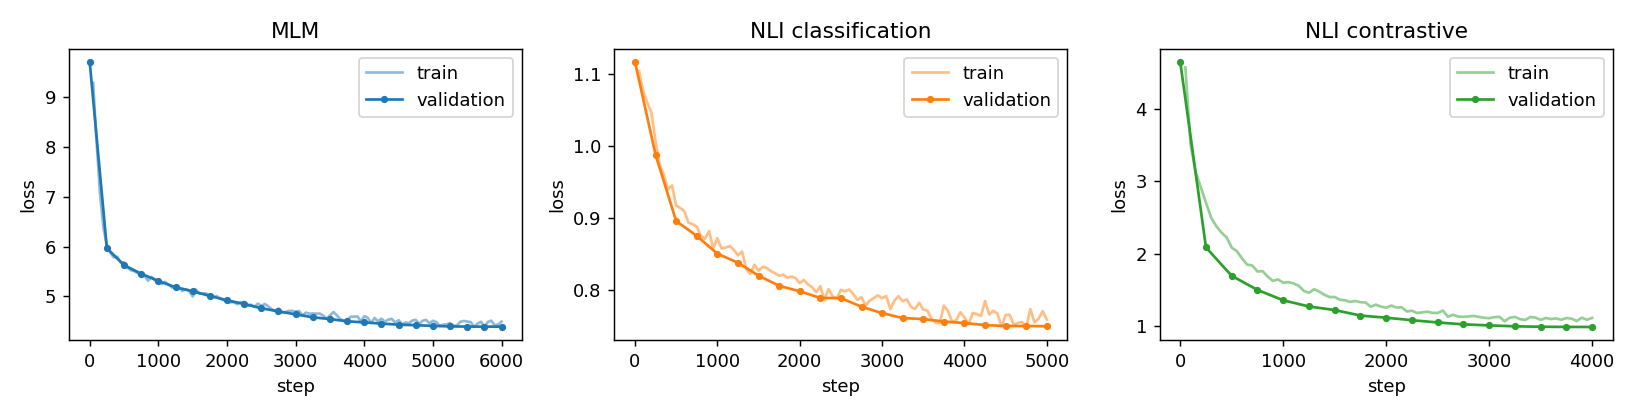
\includegraphics[width=\linewidth]{q2_loss_curves.png}\\
    {\small Training and validation loss for the three models.}
    \end{center}
    No. For all three models, the validation loss decreases and then levels
    off, and it never rises while the training loss keeps falling. It even
    ends slightly below the training loss (MLM 4.395 vs.\ 4.497, NLI
    classification 0.749 vs.\ 0.759, contrastive 0.991 vs.\ 1.116), because
    dropout is active during training but not during validation. Overfitting
    is also unlikely because none of the models completes one epoch: MLM sees
    $6000\times128\approx768$k of the 1.15M sentences, NLI classification
    640k of the 942k pairs, and the contrastive model 512k of the 558k
    triplets.

    \item \textbf{Word level vs.\ sentence level.}\par
    \begin{center}
    \begin{tabular}{lrrrr}
    \toprule
    Model & Masked-word accuracy & Similar cosine & Dissimilar cosine & Gap \\
    \midrule
    Random initialization & 10.1\% & 0.92 & 0.85 & 0.07 \\
    MLM & 34.2\% & 0.91 & 0.84 & 0.07 \\
    NLI classification & 9.2\% & 0.88 & 0.59 & 0.29 \\
    NLI contrastive & 10.1\% & 0.82 & 0.41 & 0.40 \\
    \bottomrule
    \end{tabular}
    \end{center}
    \begin{center}
    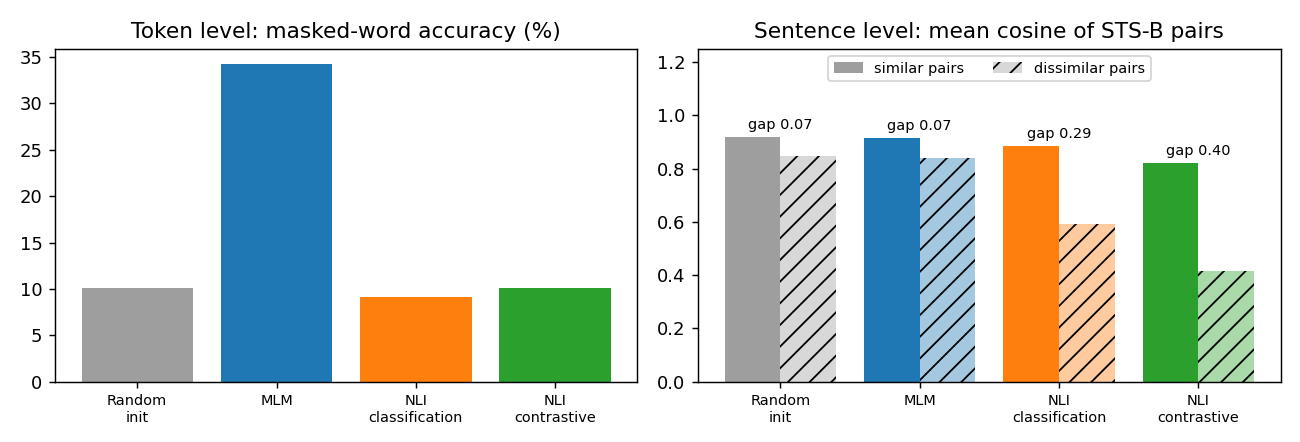
\includegraphics[width=\linewidth]{q2_evaluation.png}\\
    {\small Masked-word accuracy and mean cosine of STS-B pairs.}
    \end{center}

    \newpage
    \textbf{Fill-in-the-blank predictions} (five per model, in notebook order):

    \textit{A man is playing a [MASK].}
    \begin{itemize}
        \item Random: appointment, majoring, rejects, blinked, discharged.
        \item MLM: ball, guitar, game, bike, park.
        \item NLI classification: war, competition, married, mace, sisters.
        \item NLI contrastive: rhythm, liberty, mace, drew, instantly.
    \end{itemize}

    \textit{Two dogs are [MASK] in the snow.}
    \begin{itemize}
        \item Random: appointment, fudge, commissioner, majoring, profiled.
        \item MLM: playing, sitting, walking, standing, running.
        \item NLI classification: married, championship, painstakingly, thursdays, war.
        \item NLI contrastive: deals, outstanding, drew, smuggling, switching.
    \end{itemize}

    \textit{The chef added salt and pepper to the [MASK].} (own sentence)
    \begin{itemize}
        \item Random: appointment, blinked, pots, powder, loire.
        \item MLM: street, water, beach, city, road.
        \item NLI classification: sisters, championship, war, triple, competition.
        \item NLI contrastive: borders, commissioner, alter, remedies, 125.
    \end{itemize}

    \textbf{(a)} MLM has the highest masked-word accuracy (34.2\%), since it
    is the only model trained to predict hidden words from their context, and
    its guesses are plausible words (guitar, playing), even if not always
    right, as the chef sentence shows. The other models stay around 10\%,
    which likely matches the 10\% of selected positions left unchanged: with
    residual connections and the tied output head, an encoder not trained for
    MLM mostly predicts the input word itself.

    \textbf{(b)} NLI contrastive has the largest gap (0.40), because its loss
    directly pulls entailed pairs together and pushes the other sentences of
    the batch away in cosine space, which lowers the dissimilar cosine to
    0.41. The random and MLM encoders give a high cosine to almost every pair
    (0.84--0.92), so their mean-pooled embeddings barely separate meanings.

    \item \textbf{Classification vs.\ contrastive learning.}\par
    The following are the three highest-scoring results returned by each
    model, with their cosine similarities.

    \textit{Query: a cat is sleeping on the couch.}
    \begin{itemize}
        \item MLM: (0.95) A cat is eating corn on the cob; (0.94) A cat is playing on the floor; (0.94) A white cat stands on the floor.
        \item NLI classification: (0.93) A grey cat laying on a dining table; (0.93) Two dogs and one cat sitting on couch; (0.93) The cat is sitting on a bag of cat food.
        \item NLI contrastive: (0.70) A ginger and white cat curled up and asleep on a leather chair; (0.69) A cat sleeping on the coach with a pillow behind it; (0.62) A gray cat laying on a brown table.
    \end{itemize}

    \textit{Query: the stock market fell sharply today.}
    \begin{itemize}
        \item MLM: (0.86) But the North Korean nuclear crisis has dominated his time in office; (0.85) McGill also detailed the hole that had been cut in the Caprice's trunk; (0.84) He also reaffirmed his wish to resolve the North Korean nuclear crisis peacefully.
        \item NLI classification: (0.86) Mt Gox finds 200,000 `forgotten' bitcoins; (0.86) But Lawtey is the first entire prison to take that path; (0.85) Rogers, Videotron reach network-sharing, spectrum deal.
        \item NLI contrastive: (0.69) Also as part of the deal, PalmSource stock will begin trading on the NASDAQ stock market Wednesday under the ticker symbol: PSRC; (0.65) Shares of Corixa fell 12 cents to \$6.88 on the Nasdaq stock market; (0.57) Amazon's shares yesterday closed at \$54.32 on the Nasdaq Stock Market, up 29 cents.
    \end{itemize}

    \textit{Query: A child is playing with a dog in the park.} (own query)
    \begin{itemize}
        \item MLM: (0.94) A woman is playing volley ball; (0.93) A man is singing and playing the guitar; (0.93) A woman is playing the guitar.
        \item NLI classification: (0.96) The dog leaps over the fence in the park; (0.95) The dog plays in the park; (0.91) Some dogs running through the park.
        \item NLI contrastive: (0.80) The dog plays in the park; (0.69) The dog leaps over the fence in the park; (0.61) A kid sitting on a soccer ball at the park.
    \end{itemize}

    The contrastive loss optimizes the cosine itself against in-batch
    negatives, while classification only needs $[u;v;|u-v|]$ to be separable
    by its linear head, so its cosines stay high for every pair (0.59 for
    dissimilar pairs vs.\ 0.41) and its gap is smaller (0.29 vs.\ 0.40). The
    searches show the same thing: for the stock-market query, the
    classification model returns unrelated sentences (bitcoins, a prison) at
    0.86, while the contrastive model returns three stock-market sentences,
    and it is also the only one to find sleeping cats for the first query.

    \item \textbf{Pretraining and fine-tuning.}\par
    MLM only needs raw text (1.15M sentences here, far more in practice) and
    teaches word-level knowledge of context, as its 34.2\% masked-word
    accuracy shows, but alone it gives a poor sentence space (gap 0.07).
    Contrastive fine-tuning needs scarcer labeled pairs (558k triplets here)
    and reshapes these representations for sentence similarity (gap 0.40), so
    it comes second, starting from an encoder that already knows the language
    instead of a random one.
\end{enumerate}
}
\end{document}
